\documentclass[xcolor=dvipsnames]{beamer}

%\usetheme{Darmstadt}

\usetheme{CambridgeUS}
\usecolortheme{lily}

%\usecolortheme{beaver}

%\setbeamerfont{block title}{size={}}
%\setbeamercolor{title}{bg=blue, fg=white}
%\setbeamercolor{structure}{bg=blue, fg=white}


%\includeonlyframes{current}

\usepackage{times}
\usefonttheme{structurebold}

\usepackage{listings}
\usepackage{pgf}
\usepackage{tikz}
\usepackage{alltt}
\usepackage{verbatim}
\usepackage[normalem]{ulem}
\usetikzlibrary{arrows}
\usetikzlibrary{automata}
\usetikzlibrary{shapes}
\usepackage{amsmath,amssymb, amsxtra}
\usepackage{rotating}
\usepackage[lined,boxed,resetcount]{algorithm2e}
\usepackage{proof}
%For removing the institution name in the footers of the slides
    \defbeamertemplate*{footline}{my infolines theme}
    {
      \leavevmode%
      \hbox{%
      \begin{beamercolorbox}[wd=.333333\paperwidth,ht=2.25ex,dp=1ex,center]{author in head/foot}%
        \usebeamerfont{author in head/foot}\insertshortauthor~~\insertshortinstitute
      \end{beamercolorbox}%
      \begin{beamercolorbox}[wd=.333333\paperwidth,ht=2.25ex,dp=1ex,center]{title in head/foot}%
        \usebeamerfont{title in head/foot}\insertshorttitle
      \end{beamercolorbox}%
      \begin{beamercolorbox}[wd=.333333\paperwidth,ht=2.25ex,dp=1ex,right]{date in head/foot}%
        \usebeamerfont{date in head/foot}\insertshortdate{}\hspace*{2em}
        \insertframenumber{} / \inserttotalframenumber\hspace*{2ex}
      \end{beamercolorbox}}%
      \vskip0pt%
    }

%\setbeamercovered{dynamic}

\newcommand{\waint}{\textsc{Waint}\xspace}

\title[\waint]
{Context-Sensitive Staged Static Taint Analysis for C with LLVM}

\author[]{Xavier N. Noumbissi\\
\small{xnoumbis@uwaterloo.ca}}
\institute[2014 ECE Graduate Research Seminar]{Department of Electrical and Computer Engineering\\ University of Waterloo}
\date{}

\colorlet{redshaded}{red!25!bg}
\colorlet{shaded}{black!25!bg}
\colorlet{shadedshaded}{black!10!bg}
\colorlet{blackshaded}{black!40!bg}

\colorlet{darkred}{red!80!black}
\colorlet{darkblue}{blue!80!black}
\colorlet{darkgreen}{green!80!black}

\newcommand{\rot}[1]{\rotatebox{90}{\mbox{#1}}}
\newcommand{\gray}[1]{\mbox{#1}}
\newtheorem{prop}{Proposition}

\newcounter{myBase}
\newcounter{myCurrent}[myBase]
\setcounter{myBase}{0}
\setcounter{myCurrent}{0}

\newcommand{\inCnt}{\addtocounter{myCurrent}{1}}
\newcommand{\rstCnt}{ \stepcounter{myBase} }

%%% Command for code embedding
\newcommand{\EmbedCode}[3]{
	\lstset{language=#1}
	\lstset{basicstyle=\small,
			linewidth=10cm,
			commentstyle=\textit,
			keywordstyle=,
			stringstyle=\ttfamily,
			showspaces=false,
			numbers=#3,
			stepnumber=1,
			numberfirstline=false,
			numberblanklines=false,
			frame=none,
			showstringspaces=false,
			xleftmargin=0pt
			}
	\lstinputlisting[]{#2} 
}

\newcommand{\EmbedCodeTiny}[3]{
	\lstset{language=#1}
	\lstset{basicstyle=\tiny,
			linewidth=6cm,
			commentstyle=\textit,
			keywordstyle=,
			stringstyle=\ttfamily,
			showspaces=false,
			numbers=#3,
			stepnumber=1,
			numberfirstline=false,
			numberblanklines=false,
			frame=none,
			showstringspaces=false,
			xleftmargin=10pt}
	\lstinputlisting[]{#2} 
}

\newcommand{\EmbedCodeTinyMarg}[4]{
	\lstset{language=#1}
	\lstset{basicstyle=\tiny,
			linewidth=6cm,
			commentstyle=\textit,
			keywordstyle=,
			stringstyle=\ttfamily,
			showspaces=false,
			numbers=#3,
			stepnumber=1,
			numberfirstline=false,
			numberblanklines=false,
			frame=none,
			showstringspaces=false,
			xleftmargin=#4pt}
	\lstinputlisting[]{#2} 
}

\newcommand{\ov}[	1]{\overline{#1}}

%%for source code embedding
\definecolor{listingray}{gray}{0.9}
\definecolor{lbcolor}{rgb}{0.9,0.9,0.9}
\definecolor{forestgreen}{RGB}{34,139,34}    
\definecolor{mediumblue}{RGB}{0,0,205}    
\definecolor{firebrickred}{RGB}{178,34,34}

\begin{document}

\begin{frame}
  \titlepage
\end{frame}

%\begin{frame} \small
  %\frametitle{Outline}
  %\tableofcontents[subsectionstyle=hide]  
%\end{frame}

%%%%%%%%%%%%%%%%%%%%%%%%%% MOTIVATIONS %%%%%%%%%%%%%%%%%%%%%%%%%
\begin{frame}
  \frametitle{Problem: Prevent Software Vulnerabilities} {\Large	
	\begin{itemize}
	 \item Format String Attacks
	 \vspace{0.5cm}
	 \item SQL Injection
	 \vspace{0.5cm}
	 \item Cross Site Scripting, etc.
	\end{itemize}  
	}
\end{frame}


\begin{frame}
  \frametitle{OpenSSL Security Bug} {\large	
	\begin{itemize}
	 \item \textcolor{red}{Heartbleed} (April 7, 2014)
	 \vspace{0.5cm}
	 \item Code uses user provided buffer length without
	       checking real buffer size
	 \vspace{0.5cm}
	 \item Vulnerability gives access to server's private key
	 \vspace{0.5cm}	 
	 	 \item Could be detected by static analysis
	\end{itemize}  
	}
\end{frame}

\begin{frame}
  \frametitle{Heartbleed in OpenSSL\footnote{Image from Andy Chou's blog at Coverity}} {\large	
	\begin{center}
	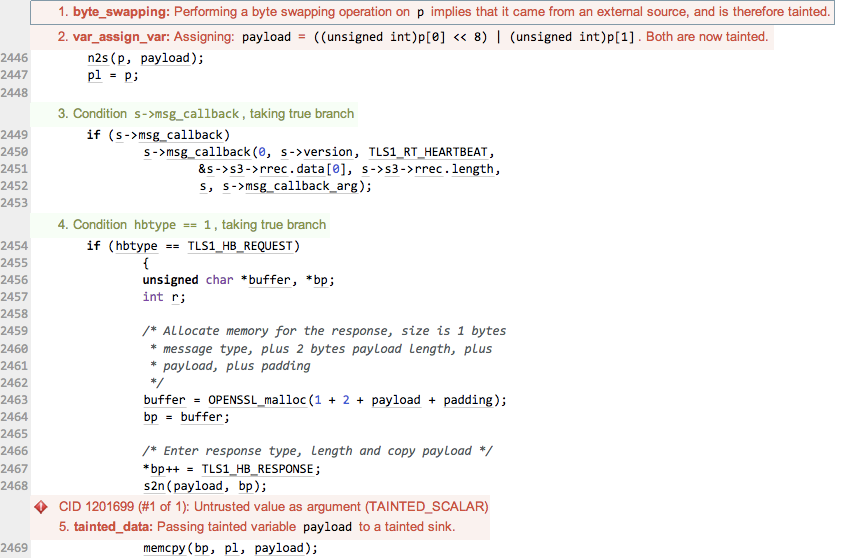
\includegraphics[scale=0.35]{heartbleed}
	\end{center}   
	}
\end{frame}

\begin{frame}
  \frametitle{Taint Analysis} {\large
   \begin{itemize}
	\item Tracks usage of untrusted program input
   	\vspace{0.5cm}	   
	\item Untrusted program input: \textcolor{red}{Tainted Input}
   	\vspace{0.5cm}	
	\item \textcolor{forestgreen}{Taint source}: tainted input origin (e.g. system call return values)
   	\vspace{0.5cm}
	\item \textcolor{forestgreen}{Taint sink}: use of tainted input
	\end{itemize}
	}
\end{frame}

\begin{frame}
  \frametitle{Taint Analysis: taint propagation} {\large
   \begin{itemize}
   	\item \textcolor{forestgreen}{Taint propagation}: operations depending on tainted input generate tainted values
   	\vspace{0.5cm}	   	
   	\item Explicit taint propagation: \textcolor{blue}{data flow}
   	\vspace{0.5cm}	
	\item Implicit taint propagation: \textcolor{blue}{control flow}   	
	\end{itemize}
	}
\end{frame}


\begin{frame}
  \frametitle{Example} 
    {\small
    \begin{center}
	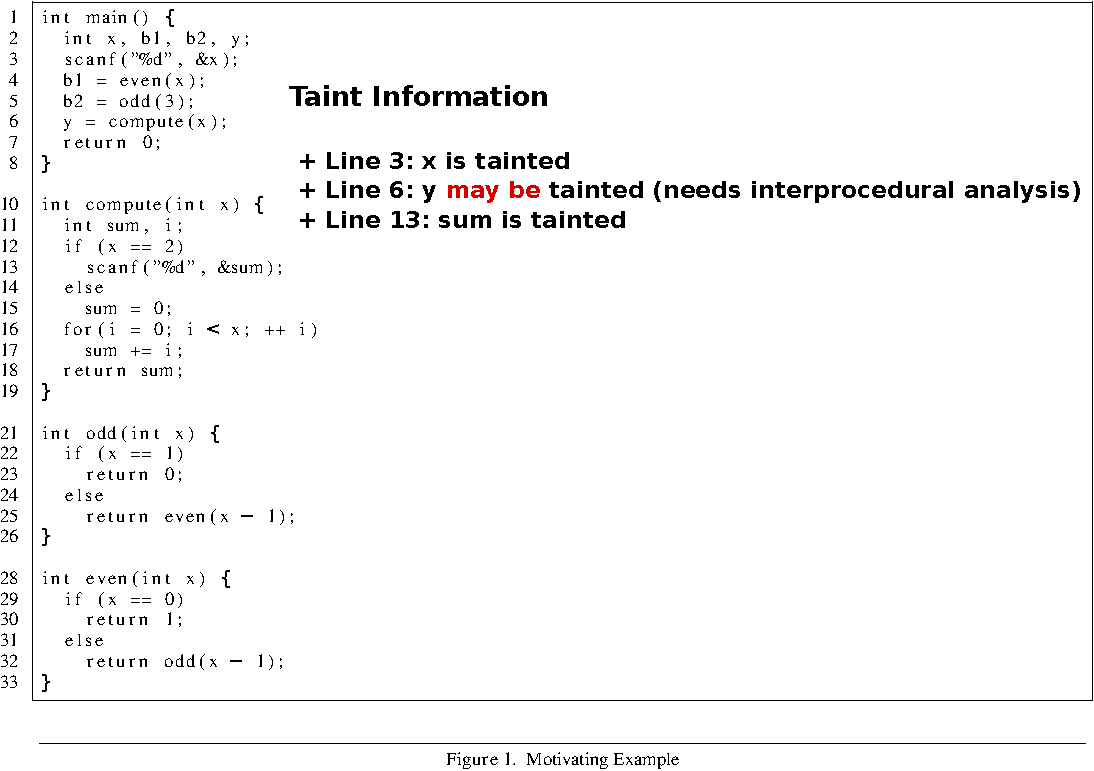
\includegraphics[scale=0.6]{example-explained}   	
	\end{center}   
	}
\end{frame}

\begin{frame}
  \frametitle{Contributions} 
	{\large
	\begin{itemize}
	\item Algorithm to statically detect tainted values' flow in C programs
   	\vspace{0.5cm}
	\item Handling of interprocedural taint propagation
   	\vspace{0.5cm}   	
	\item \waint: Implementation of the algorithm in LLVM
	\end{itemize}
	}
\end{frame}

\begin{frame}
  \frametitle{Source/Sink Specification} 
    {\large
	\begin{itemize}
	\item Developer specify sources and sinks in configuration file
   	\vspace{0.5cm}	
   	\item Analysis do not analyze sources and sinks
   	\vspace{0.5cm}	     	   		   	
   	\item Analysis use annotations for sources: taint propagation (from configuration file)
   	\end{itemize}
	}
\end{frame}

\begin{frame}
  \frametitle{\waint Analysis} 
	{\large
	\begin{itemize}	
   	\item Summary table to store function parameters and return value taint information
   	\vspace{0.5cm}   	
	\item Intraprocedural analysis: discovery of taint sources, initial values
	for summary table
   	\vspace{0.5cm}	   	
	\item Context-Sensitive analysis: interprocedural taint tracking using
	DSA alias analysis
   	\vspace{0.5cm}		   	
	\item Context-Insensitive analysis: use summary table information
	\end{itemize}
}
\end{frame}

\begin{frame}
  \frametitle{\waint Analysis (Flow)} 
	{\small
	\begin{center}
	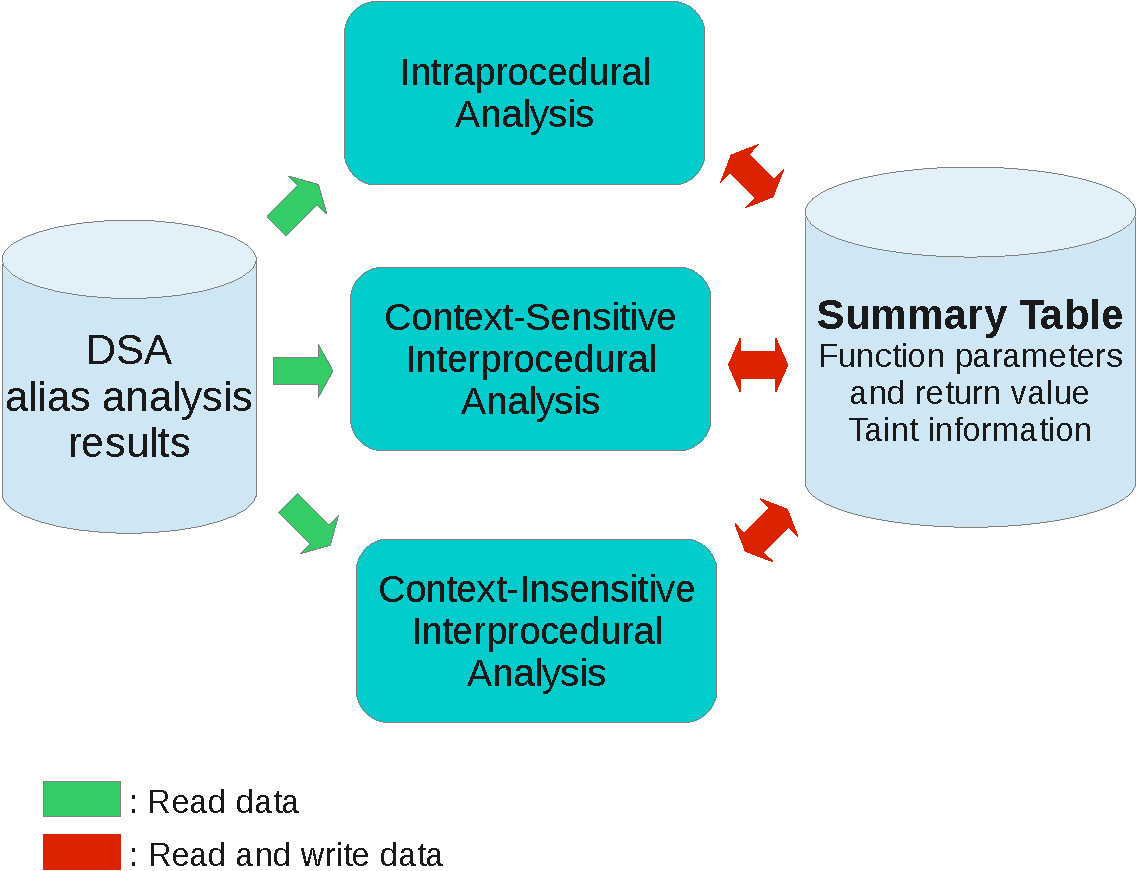
\includegraphics[scale=0.4]{analysisFlow}
	\end{center}  	
}
\end{frame}

\begin{frame}
  \frametitle{Intraprocedural Analysis} 
	\Large
\begin{center}
\begin{tabular}{|l|l|}
\hline
Statement Type 				& C Code 			\\ \hline
\hline
\textcolor{blue}{COPY}		& $p = q$				\\	\hline
\textcolor{blue}{LOAD}		& $p = *q$				\\ 	\hline
\textcolor{blue}{STORE}		& $*p = q$				\\ 	\hline
\textcolor{blue}{CALL}		& $\mathit{call\ func}  $ \\ 	\hline
\end{tabular}
\end{center}    	
\end{frame}

\begin{frame}
  \frametitle{Intraprocedural Analysis: transfer functions} 
	{\large
	\begin{itemize}
	\item \textcolor{blue}{COPY}\ [$p = q$]: \textcolor{red}{taint p} iff q is tainted
   	\vspace{0.2cm}	
	\item \textcolor{blue}{LOAD}\ [$p = *q$]: \textcolor{red}{taint p} iff $t_q = *q \wedge t_q$ is tainted
   	\vspace{0.2cm}		
	\item \textcolor{blue}{STORE}\ [$*p = q$]: \textcolor{red}{taint $t_p$} $= *p$ iff q is tainted
   	\vspace{0.2cm}				
	\item \textcolor{blue}{CALL}\	 [$\mathit{call\ func(p)}$]: \textcolor{red}{taint all} $t_p\ \mathtt{s.t}\ t_p = *p$ 
	\end{itemize}
}
\end{frame}

\begin{frame}
  \frametitle{Example (2)} 
    {\small
    \begin{center}
	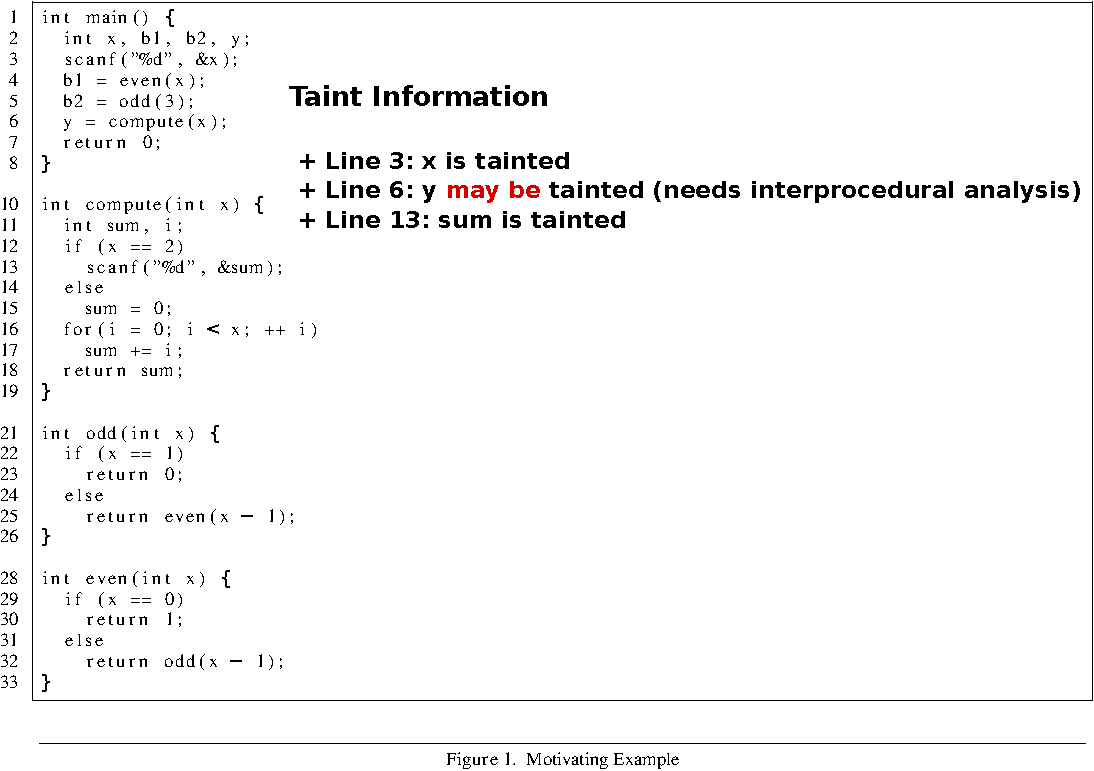
\includegraphics[scale=0.6]{example-explained}   	
	\end{center}   
	}
\end{frame}


\begin{frame}
  \frametitle{Summary Table after Intraprodural Analysis} 
	\Large
\begin{center}
\begin{tabular}{|l|l|}
\hline
Functions 							& 	Variables 					\\ \hline
\hline
\textcolor{forestgreen}{even}		& 	$x^u$, $\mathit{ret}^u$		\\	\hline
\textcolor{forestgreen}{odd}		& 	$x^u$, $\mathit{ret}^u$		\\ 	\hline
\textcolor{forestgreen}{compute}	& 	$x^u$, $\mathit{ret}^t$		\\ 	\hline
\textcolor{forestgreen}{main}		& 	$ret^u$						\\ 	\hline
\end{tabular}
\end{center}    	
\end{frame}

\begin{frame}
  \frametitle{Context-Sensitive Analysis} {
   \large
   \begin{itemize}
   \item Same transfer functions as intraprocedural analysis except \textcolor{blue}{CALL}
	\vspace{0.2cm}   
   \item Use Data Structure Analysis (DSA): field- and context-sensitive alias
   analysis\footnote{from LLVM creator Chris Lattner}
	\vspace{0.2cm}   
   \item Analysis of a callee start with taint assumptions from the caller
	\vspace{0.2cm}      
   \item Use summary table for procedure formals and return value initial taint information
   
	\end{itemize}
	}
\end{frame}

\begin{frame}
  \frametitle{Context-Insensitive Analysis} {
   \Large
   \begin{itemize}
   \item Use functions' return value taint information from summary table
	\vspace{0.5cm}   
   \item In practice: useful after context-sensitive analysis
   
	\end{itemize}
	}
\end{frame}

\begin{frame}
  \frametitle{Example: \waint} 
    {\small
    \begin{center}
	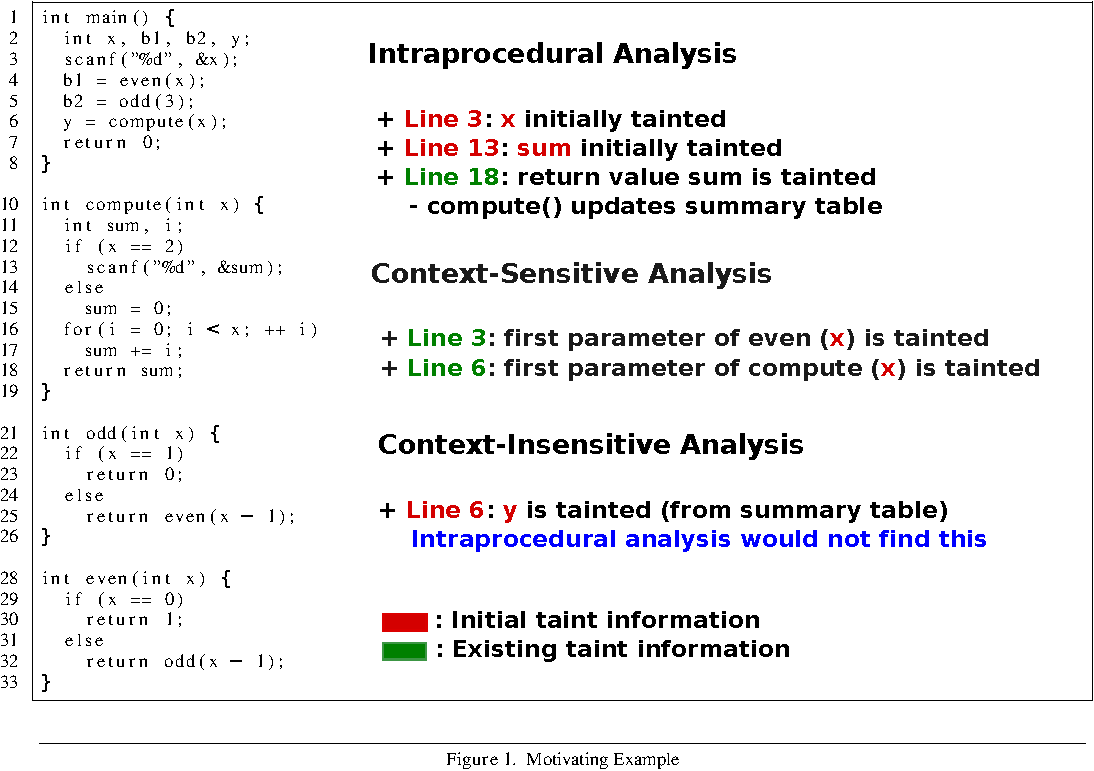
\includegraphics[scale=0.55]{example-waint}   	
	\end{center}   
	}
\end{frame}

\begin{frame}
  \frametitle{Current Implementation}
   \small
\begin{center}
\begin{tabular}{|l|l|c|c|}
\hline
\textbf{Program} 			& \textbf{SLOC}	&	\textbf{Warnings}	&	\textbf{Runtime}		\\ \hline
\hline
Mongoose web server (4.1)	& $4k$	&	$36$		&	$140$s		\\	\hline
vlc-input (2.1.2)			& $16k$ &	$0$			&	$6$s		\\ \hline
Claws email client (3.9.3)	& $142k$&	$219$		&	$11$s		\\ 	\hline
Apache web server (2.4.7)	& $144k$&	n/a			&	n/a (DSA crash) \\ 	\hline
\end{tabular}
\end{center} 
\end{frame}

\begin{frame}
  \frametitle{TODOs/Future Work} 
    {\Large
   \begin{itemize}
   \item Handling of arrays, structs
	\vspace{0.5cm}   
   \item Handling of cycles (SCC) in call graph
	\vspace{0.5cm}      
   \item Investigate crash of DSA while running Apache   
	\vspace{0.5cm}      
   \item Perform tests with other alias analysis      
	\end{itemize}
	}
\end{frame}

\begin{frame}
  \frametitle{Conclusion} {
   \Large
	\begin{itemize}
	\item \textbf{Hearbleed} bug in OpenSSL shows importance of taint analysis
	\vspace{0.5cm}	
	\item \waint implements a context-sensitive taint analysis for C
	\vspace{0.5cm}
	\item Preliminary results scale well up to $150k$ lines of code
	\end{itemize}   
	}
\end{frame}


\end{document}
